\documentclass[12pt]{article}
\usepackage{amsmath}
\usepackage{amssymb}
\usepackage[utf8]{inputenc}
\usepackage[english]{babel}
\newcommand{\R}{\mathbb{R}}
\usepackage{graphicx}
\setlength{\parindent}{0pt}% Just for this example

\title{Algorithmic Operation Research \\ Homework 2}
\date{25-10-2019}
\author{Theodora Panagea - 1115201400135 \\ Anna-Aikaterini Kavvada - 1115201500050}

\begin{document}
	\maketitle{}
  	\pagenumbering{arabic}
  	
%-------------------Exercise 1--------------------------

\subsection*{Exercise 1}
Find a differentiable function $f: \R \rightarrow \R$ such that $f$ does not have an extremum at its critical point. \\
\textbf{Solution:} \par

\newpage

%-------------------Exercise 2--------------------------

\subsection*{Exercise 2}
Given a positive integer $S$, which decompositions  \\
$$a_1+\cdots+a_n = S$$ \\
with the $a_i$ positive integers have the largest product $a_1 \cdots a_n$ ? \\
\textbf{Solution:} \par

\newpage

%-------------------Exercise 3--------------------------

\subsection*{Exercise 3}
Find the optimal solution to the Diet Problem when the cost function is \\
$$Cost(x_1, x_2) = x_1 + x_2.$$
\textbf{Solution:} \par

\newpage

%-------------------Exercise 4--------------------------

\subsection*{Exercise 4}
 Let $A, B \in \R^{nxn}$. Show that the traditional way of computing their product $AB$ requires a total of $(2n-1)n^2$ arithmetic operations.\\
\textbf{Solution:} \par

\newpage

%-------------------Exercise 5--------------------------

\subsection*{Exercise 5}
Consider the problem of solving a system of $n$ linear equations in  $n$ unknowns. Show that the Gaussian elimination method requires $\mathcal{O}(n^3)$ arithmetic operations in order to either compute a solution or to decide that no solution exist.\\
\textbf{Solution:} \par

\newpage

%-------------------Exercise 6--------------------------

\subsection*{Exercise 6}
Suppose that we are given a set of vectors in $\R^n$ that form a basis and let $y$ be an $n$ arbitrary vector in $\R^n$. We wish to express $y$ as a linear combination of the basis vectors. How can this by accomplished?\\
\textbf{Solution:} \par

\newpage

%-------------------Exercise 7--------------------------

\subsection*{Exercise 7}
Study the paper with title: "Do dogs know Calculus?" found in the Readings folder.\\
\textbf{Solution:} \par
{Below follows a small presentation of the paper "Do dogs know claculus", written by Timothy J.Pennings.\\
The problem this paper refers to can be categorized as an \textit{optimal path} problem. For a path to be optimal, it may be that we minimize the travel time between the two points (start point (A), end point (B)), while taking into consideration that the available paths must transverse two different mediums, involving different rates in speed.\par 
In this paper, we apply the above on Elvis' case (Elvis' being the author's corgi). Thus, we have Elvis who seems to be determined every time to fetch his ball as quickly as possible, without caring about the energy expenses he might suffer. This, leads us to the assumption that Elvis, unconciously tries to "calculate" the optimal path to minimiae the balls retreival time.\par 
\begin{center}
\textbf{The situation}
\end{center}
We are standing on the water's edge (point A) of Lake Michigan to play fetch the ball with Elvis. After the tennis ball we use, ends up at point B, as shown in the figure below.
\begin{figure}[h!]
  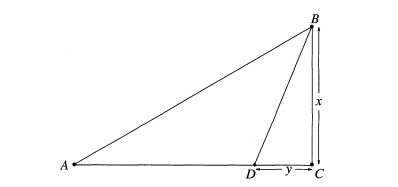
\includegraphics[width=\linewidth]{pathsToTheBall.png}
  \caption{Paths to the ball.}
  \label{fig:path1}
\end{figure}
\begin{center}
\textbf{What is Elvis' strategy?}\\  
\end{center}
$\textbf{1.}$ Minimize retrieval time by minimizing the distance\\
$\textbf{2.}$ Minimize swimming distance since $u_{run} > u_{swim}$ \\
$\textbf{3.}$ Running a portion of the way and swimming the rest \\ $\newline$
\textbf{Note:}Option 3, usually turns out to minimize the time (depends on the relative $u_{run}$ and $u_{swim}$)
\begin{center}
\textbf{Solve the problem $\rightarrow$ General Case}\\
\end{center}
$\bullet r = u_{run}$: running speed\\
$\bullet s = u_{swim}$: swimming speed\\
$\bullet$ units used: meters and seconds\\
$\bullet T(y)$:time to get to the ball, given that Elvis jumps into the water at D\\
$\bullet z = (AC)\newline$\\ 
We have\\ $$\newline T(y) = \frac{z-y}{r} + \frac{\sqrt{x^2 + y^2}}{s} \quad (1)$$\\
For $T'(y)= 0$, we calculate the minimum value for the equation. Solving $T'(y) = 0$ for $y$, we get 
$$y  = \frac{x}{\sqrt{\frac{r}{s}+1}\sqrt{\frac{r}{s}-1}} \quad (2)\newline$$\\ 
\textbf{Note:} T is seen to have a minimum by using the second derivative set.\newpage
\begin{center}
\textbf{Notices}\\
\end{center}
$\textbf{1.}$ The optimal path does not depend on $z$, while $z>y$ \newline
$\textbf{2.}$ If $r<s$, the problem cannot be solved\newline
$\textbf{3.}$ $\bullet r \gg ss \rightarrow y$ is small \newline $\bullet r \approx s \rightarrow y$ is large\\
$\textbf{4.}$ $r,s \rightarrow$ fixed $\rightarrow y$ is proportional to x\\

\begin{center}
\textbf{Return to Experiment}\\
\end{center}
While playing, we see Elvis: \\

$\bullet$choosing option $3$ of jumping into the lake at point D\\
$\bullet$ $y$ values being proportional to $x$ values\\

Thus, after timing Elvis' performance, we get the table below\\
\begin{figure}[h!]
  \begin{center}
  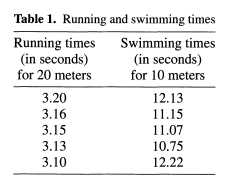
\includegraphics[width=50mm]{experimentTable.png}
  \label{fig:path1}
  \end{center}
\end{figure}\\
After the trials above, we choose the three optimal running and swimming times for Elvis and get their average $$r=6.4m/s \quad and \quad s=0.910m/s$$.\\
Then we have $$(2) \Rightarrow y = 0.144x \quad (3)$$\\ \newpage
Following the above preparation, is the experiment. Below there is the table of Elvis' throw and fetch trials and the scatterplot of the tables data.  
\begin{figure}[h!]
  \begin{center}
  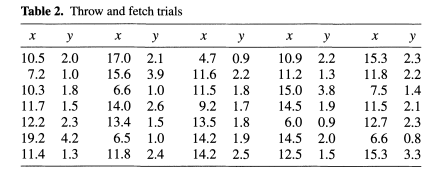
\includegraphics[width=100mm]{throwFetchTrials.png}
  \label{fig:path2}
  \end{center}
\end{figure}\\

\begin{figure}[h!]
  \begin{center}
  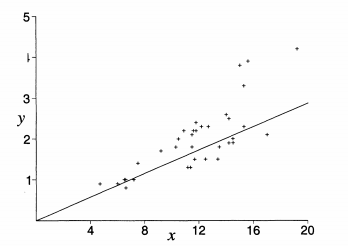
\includegraphics[width=100mm]{ElvisChoice.png}
  \caption{Scatter Plot of Elvis's choices with optimal line}
  \label{fig:path3}
  \end{center}
\end{figure}\\

In figure 2 we clearly see that most of the points show a rather tight and clear pattern, or as statisticians would call it, smooth. \\In the same figure we also see the line we predicted from the model we created, $y = 0.144x.$ \newpage
\begin{center}
\textbf{Assumptions}\\
\end{center}
\textbf{1.}There was a definite line between shore and lake. Because of waves, this
was not the case\\
\textbf{2.}When Elvis entered the water, he started swimming. Actually, he
ran a short distance in the water.\\
\textbf{3.}The ball was stationary in the water\\
\textbf{4.}The values of r and s are constant, independent of the distance run
or swum.\\ \\
\textbf{Note:} There is the possibility that Elvis chose paths actually \textit{better} than the optimal we predicted\\
\begin{center}
\textbf{Conclusion}\\
\end{center}
\textbf{1.} We use a mathematical model.\\
\textbf{2.} To arrive at the theoritical figure we made all of the above simplifying assumptions\\
\textbf{3.} There is always the possibility of an error in measurements\\

However, despite all of the above, Elvis does not know calculus. In fact, he has trouble differentiating even simple polynomials. More seriously,
although he does not do the calculations, Elvis's behavior is an example of the uncanny way in which nature (or Nature) often finds optimal solutions. Consider how
soap bubbles minimize surface area, for example. It is fascinating that this optimizing
ability seems to extend even to animal behavior. (It could be a consequence of natural selection, which gives a slight but consequential advantage to those animals that
exhibit better judgment.) 
}

\end{document}  	